\section{Implémentation de la solution}
Plusieurs des solutions que nous avons testées ne nous ont pas permis d'atteindre l'objectif du projet.
Par exemple, nous n'avons pas retenu l'algorithme de Canny, qui malgré plusieurs traitements sur l'algorithme
de base, ne permettait pas de s'abstraire de la luminosité de la vidéo.
Nous allons donc voir en détail les solutions qui ont été utilisées pour atteindre nos objectifs.

\subsection{Solutions utilisées dans l'application}
Lorsque nous analysons une vidéo pour en extraire le centre de l'oeil, nous sommes confrontés à certaines contraintes.
Cependant, la majorité d'entre elles dépendent de la gestion de la couleur de l'image que nous analysons. C'est
pourquoi l'algorithme de Canny n'était pas efficace, car celui-ci était appliqué à une image en dégradé de gris
et donc subissait les effets de la luminosité de la vidéo.\\

Nous avons donc choisi d'utiliser un modèle colorimétrique différent afin d'en extraire une des composantes.
Notre solution utilise le canal de la première chrominance du modèle colorimétrique YCbCr ce qui permet 
de ne plus prendre en compte la couleur de peau et de diminuer l'effet de la luminosité dans l'image que nous traitons.\\

%TODO binarisation

Une fois la binarisation effectuée, nous devons détecter la forme de l'oeil. Pour cela, nous utilisons les blobs, qui nous
permettent non seulement de récupérer des enveloppes convexes présentes dans l'image, mais aussi de déterminer quelle enveloppe
correspond à l'oeil. Pour cela, nous vérifions que l'enveloppe convexe est celle qui est la plus au centre.
Nous calculons ensuite le barycentre de cette forme afin d'obtenir le centre de l'oeil.\\

Cette solution ne gère pas complètement le cas où l'oeil de l'utilisateur est fermé. Dans le cas où notre algorithme
n'arrive pas à calculer le centre de l'oeil, nous récupérons les coordonnées du point qui étaient calculées par la méthode 
de l'équipe. Ainsi, dans le cas où nous ne détectons aucun blob, nous obtenons tout de même un point, sauf si la méthode 
précédente ne fonctionne pas non plus.

\subsection{Comparaison des résultats obtenus avec les anciens résultats}
Afin de valider nos travaux, nous avons pu tester nos points sur des vidéos comportant les points correspondants à
la vérité terrain. Pour comparer les points de l'ancienne méthode avec les nôtres, nous calculons la
distance entre ces points et la vérité terrain.\\

Pour avoir des éléments de comparaison, nous faisons la moyenne de ces deux distances pour une vidéo, et nous calculons
le nombre de cas dans lesquels nos points sont plus efficaces. Dans la première vidéo nous obtenons 70\% de points plus précis, et
60\% pour la seconde vidéo.\\

\begin{figure}[H]
  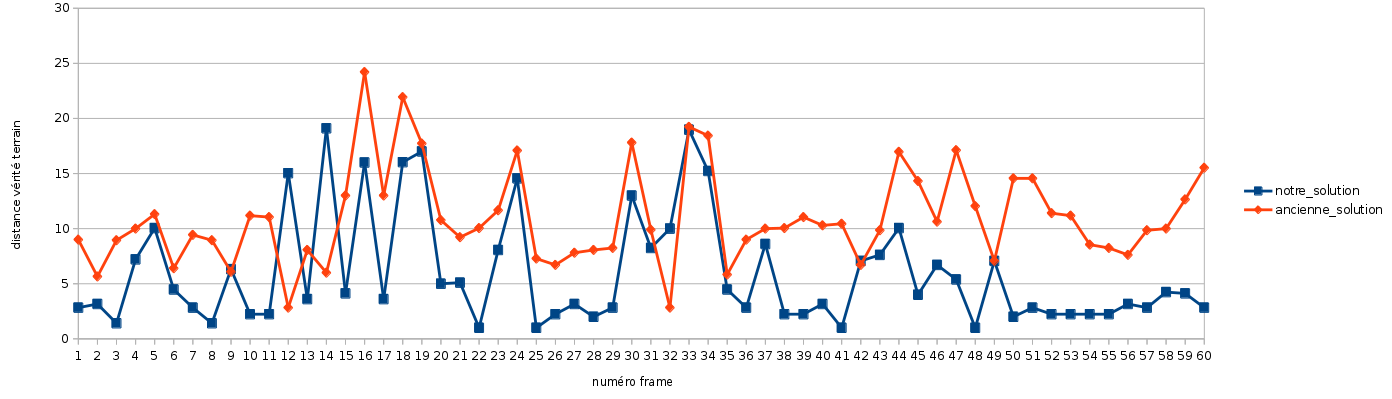
\includegraphics[width=17cm]{resultat/resultat_gauche.png}
  \caption{Comparaison des résultats pour l'oeil gauche}
\end{figure}

\begin{figure}[H]
  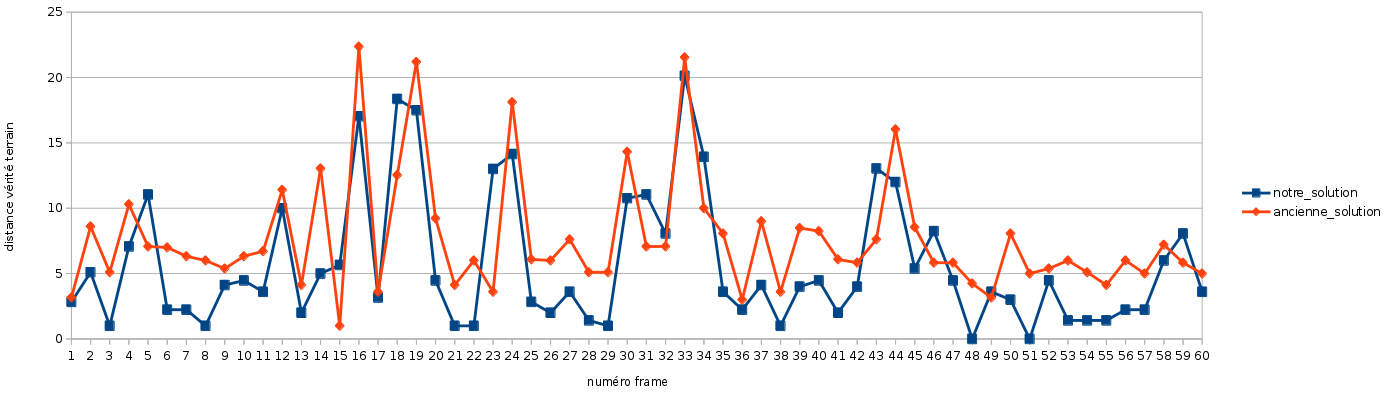
\includegraphics[width=17cm]{resultat/resultat_droit.png}
  \caption{Comparaison des résultats pour l'oeil droit}
\end{figure}

%Avec cette méthode, nous obtenons les résultats présents dans l'annexe p\pageref{resultatApplication}. 
Nous pouvons voir que notre algorithme est plus efficace, en sachant que dans le cas où il ne détecte pas de point, il se repose sur l'ancien
calcul. De plus, nous avons pu constater que la condition que nous posons sur la sélection du blob peut poser problème 
avec le sourcil de la personne quand le blob du sourcil et celui de l'oeil sont à égale distance du centre de la fenêtre.\\

Notre solution améliore donc légèrement la position du centre de l'oeil détecté par l'algorithme de l'équipe FOX. Certaines
situations ne sont pas encore bien gérées dans l'application, mais nous avons pu étudier quelques solutions qui pourraient améliorer
la localisation de l'oeil.

\subsection{Améliorations envisageables}
Tous les objectifs n'ont pas été remplis, car la recherche de solution pour l'optimisation du calcul du centre de l'oeil
nous a pris beaucoup de temps à cause des pistes qui n'ont pas abouti. Notre point obtient de meilleurs résultats
que celui utilisé précédement, mais il reste toujours un écart avec la vérité terrain. \\Il est donc encore possible
d'améliorer notre solution.\\

Le second objectif sur la localisation de l'oeil, lorsque celui-ci est fermé, n'est pas abouti. Notre solution
nous permet de détecter parfois un point dans ce cas. Mais ce qu'il trouve n'est pas le centre de l'oeil mais le
centre des cils qui sont plus visibles lorsque les yeux sont fermés.
%TODO